\documentclass[portrait,10pt]{article}
\usepackage{graphicx} %Use this for \includegraphics[]{}
\usepackage{float}
\usepackage[margin=1in,showframe=false]{geometry}
\usepackage{longtable}
\usepackage{hyperref}
\usepackage{stmaryrd}
\usepackage{keystroke}
\usepackage{textcomp}
\usepackage{MnSymbol}
\usepackage{amsmath}
\usepackage{epigraph}
\begin{document} %What do you think?

\date{\today}
\title{SciDraw: A Quick-Start Guide to Make Level Schemes}
\author{Clark Casarella}
\maketitle
\section{Impetus For This Guide}

The purpose of this tutorial is to provide a concise, straightforward method to begin making simple, publication quality level schemes for nuclear physics. This guide is \textit{not} meant to replace M. Caprio's complete and exhaustive guide, examples, or built-in documentation delivered with the SciDraw distribution, but will provide the barebones knowledge on how to go from no level scheme to a non-zero number of level schemes in a quick fashion.
\section{Installing SciDraw with Wolfram Mathematica 9.0+}

Use of M. Caprio's SciDraw package for Mathematica assumes a few things: a) the user has downloaded and installed Wolfram Mathematica for his/her computer (a software license can be obtained from \url{http://oit.nd.edu}'s software download page for undergraduates, graduate students, and faculty), b) the user has downloaded the latest SciDraw distribution from M. Caprio's webpage at Notre Dame. (\url{http://scidraw.nd.edu/}) provides the web URL (as of April 29, 2016) for users that printed this tutorial and a hyperlink to the URL for individuals with this \textit{pdf} distribution. On this page, there is a link to the latest release(s) of SciDraw, and download the latest .zip release (as of April 29, 2016, \textit{SciDraw-0.0.7.zip}) to your local machine. 

Next, we must tell Mathematica to look for SciDraw in a particular location to use this custom package set. Inside the \textit{.zip} archive, there are several folders, all of which need to be extracted to one of two locations on your machine: the Mathematica Applications directory (where the installation files for Mathematica exist), or to any other (easily accessible) directory. Unzipping the archive to the Applications folder is generally the more difficult of the two options, especially if the current user does not have root access to view/edit hidden files associated with the Mathematica installation. My preferred method is obviously the latter of the two, pending ease of instruction across multiple Operating Systems.

With the archive unpacked \textit{somewhere}, open a new Mathematica notebook and type: 
\[
{\tt \$UserBaseDirectory}
\]
For those unfamiliar with the workings of Mathematica, any command in Mathematica is executed by pressing the SHIFT+ENTER/RETURN keys (\Shift+\Enter or \Shift+\Return, depending on your keyboard layout). Execute this {\tt \$UserBaseDirectory} command, and Mathematica will produce an output that tells you the location of your Mathematica executable(s). This output is different for the user and Operating System, but as an example, my \$UserBaseDirectory is:
\[
/home/clarkc/.Mathematica
\]
Navigate to this directory and open the `Kernel' directory; inside that, you will find a single file, `\textit{init.m}'. Open this file with a text editor and you should see a mostly empty file, where you will need to specify the path to the SciDraw folder you extracted from the archive. To do this, type (anywhere in the init.m file):

\[
{\tt AppendTo[\$Path,``\sim/path/to/SciDraw/folder/"];}
\]
Here, the ``$\sim$/path/to/SciDraw/folder" should be the directory path to the SciDraw folder. \textbf{IMPORTANT NOTE:} this path must be the path that includes the folders ``BlockOptions", ``CustomTicks", ``InheritOptions", among others. This must be in double quotations, and the formatting is somewhat dependent on the user's Operating System. Mac OS and Linux users will use the standard forward slash when specifying a path ({\tt "$\sim$/clarkc/Desktop/SciDraw/"}), while Windows users need to use a double backslash to separate folders ({\tt "C:$\backslash\backslash$Users$\backslash\backslash$clarkc$\backslash\backslash$Downloads$\backslash\backslash$SciDraw"}). Save and close this \textit{init.m} file, and restart Mathematica completely; Mathematica will now automatically look in the location to find SciDraw, which we must initialize before the user can start drawing.

\textbf{To summarize:}
\begin{enumerate}
\item Install Mathematica 9.0+
\item Download SciDraw and extract the contents to a location
\item Find the \textit{init.m} file from the Mathematica Kernel with {\tt \$UserBaseDirectory}
\item Use the {\tt AppendTo} command to point to the location of SciDraw on your machine
\item Save the \textit{init.m} file, and restart Mathematica
\end{enumerate}
\subsection{Initializing SciDraw}

SciDraw must be called into use by Mathematica before the user can start generating level schemes, and must only be done once for a particular session of Mathematica. Any STOP to the local computational kernel of Mathematica will also stop/close SciDraw, and must be re-loaded. Luckily, a kernel STOP is uncommon, meaning it is done manually, and is \textit{generally never done by accident}. To load SciDraw in a Mathematica notebook, type:
\[
{\tt <<SciDraw^\backprime}
\]

Take special care to not forget the \keystroke{$^\sim\backprime$} (the grave accent/tilde key above \Tab on most keyboards) keystroke at the end of the command. One this command is executed, you will see a small splash screen:

\begin{figure}[h]
\begin{center}
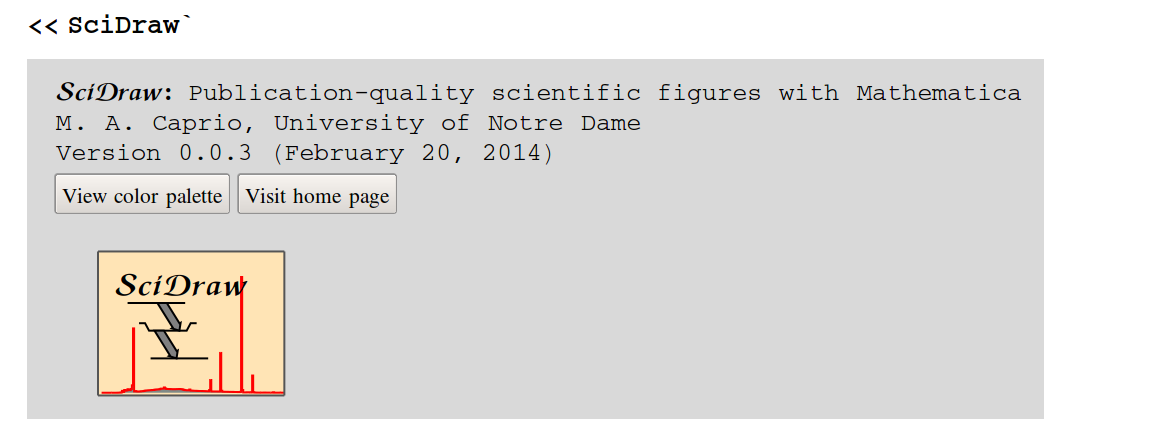
\includegraphics[width=0.70\textwidth]{SciDraw_splash.png}
\caption{SciDraw splash screen inside Mathematica, indicating that the package has been loaded for use.\label{fig:splash}}
\end{center}
\end{figure}

Once the package has been loaded (remember to insert this command at the top of \textit{every} separate Level Scheme file you want to use), you are now ready to make level schemes!
\section{Drawing Figures/Level Schemes in SciDraw}

Included with this guide distribution, there is a Mathematica notebook to serve as a template, or minimally working example, for the user's convenience. The remainder of this guide serves to outline what each command in the template will do, with explanations on the syntax.
\subsection{Preparing the Canvas and FigurePanel}

Level schemes are drawn onto a Canvas of some set size, and in Mathematica, this is done by making a {\tt Figure[ ];}, which only needs the {\tt CanvasSize$\rightarrow$F$_{scale}$*\{x,y\}} argument to state how large the image will be, with F$_{scale}$ being a final image scaling factor applied to the aspect ratio ({\tt \{x,y\}}). Inside the figure, we must then place at least one {\tt FigurePanel}, as SciDraw can place multiple inset plots onto a canvas (this is an advanced user option, refer to M. Caprio's full documentation). Each {\tt FigurePanel} needs a {\tt PlotRange$\rightarrow$\{\{x$_{min}$,x$_{max}$\},\{y$_{min}$,y$_{max}$\}\}}, the range over where the plot is displayed. To make a canvas that is 100\% size and 4:3 aspect ratio with a single, empty plot from x$\in$\{0,1\} and y$\in$\{-10,100\}, type the text from Figure \ref{text:blankcanvas} into Mathematica.

\begin{figure}[h]
\begin{tt}
Figure[\\
 FigurePanel[\\
  $\{$\\
   \\
   $\}$,\\
  PlotRange $\rightarrow$ $\{\{$0, 1\}, $\{$-10, 100$\}\}$\\
  \\
  ];,\\
 CanvasSize $\rightarrow$ 1.00*$\{$4, 3$\}$\\
 ]\\
\end{tt}
\begin{center}
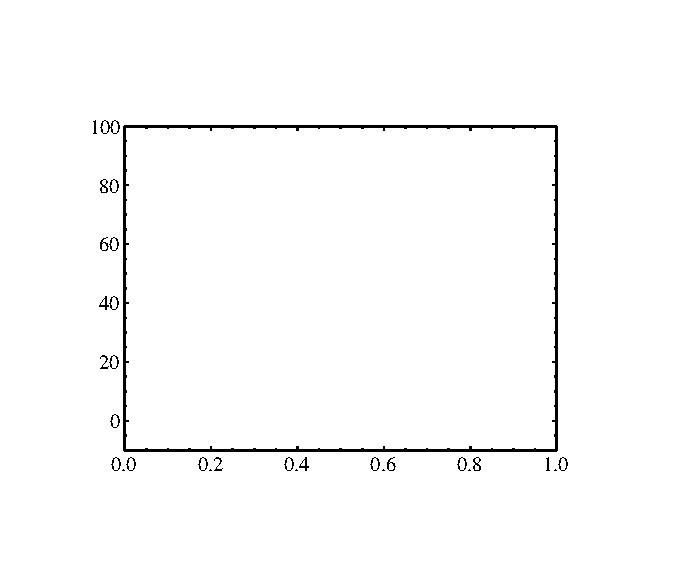
\includegraphics[width=0.5\textwidth]{BlankCanvas.eps}
\end{center}
\caption{Blank SciDraw canvas. The `$\rightarrow$' is \keystroke{-} followed by \keystroke{$>$} in Mathematica. \label{text:blankcanvas}}
 \end{figure}

\textbf{A note going forward:} All commands to make objects (levels, transitions, labels, \textit{etc}) are placed in the `body' of the {\tt FigurePanel} (inside the curly brackets).
%PlotRange
%XYFrame
%FrameLabel
%CanvasMargin
\subsection{Adding Levels to the Figure}

A level scheme without levels is just a scheme, no? We will now place a level, the fundamental object every command in the remainder of this guide will use, reference, or be anchored to. Levels require only a few inputs: a) a name to reference it by (``{\tt Level\_Name}"), b) a position on the x-axis where the level begins ({\tt x$_0$}), c) a position on the x-axis where the level ends ({\tt x$_1$}), d) the position on the y-axis where the level lies ({\tt E$_{{\tt lev}}$}), and optionally, e) any options to modify the level (\textit{options}). Options for levels, transitions, and labels are discussed at the end of the document and are \textit{always} optional. To draw a level, use the 'Lev' command inside the FigurePanel:

\begin{equation} \label{eq:Lev}
{\tt Lev\llbracket``Level\_Name"\rrbracket[x_0,x_1,E_{lev},\textit{options}];}
\end{equation}

A note to the user, SciDraw automatically places a margin of length 0.1 on every level. For example, a level drawn from {\tt x$_0$}=`0' to {\tt x$_1$}=`1' will really be drawn from 0.1 to 0.9; this is done to aid the user to allow sufficient room for small labels on the side with ease. The $\llbracket$ and $\rrbracket$ are done by simply typing two square brackets (\keystroke{{\tiny $^\{$[}}\keystroke{{\tiny $^\{$[}} and \keystroke{{\tiny $^\}$]}}\keystroke{{\tiny $^\}$]}}). Adding:

\begin{figure}[h!]
\begin{center}
{\tt Lev$\llbracket``$162Dy$\_$0gs$"\rrbracket$[0,1,0];}\\
\end{center}
Inside the `\{' `\}' of {\tt FigurePanel[ \{ \}, ];} will produce:\\
\begin{center}
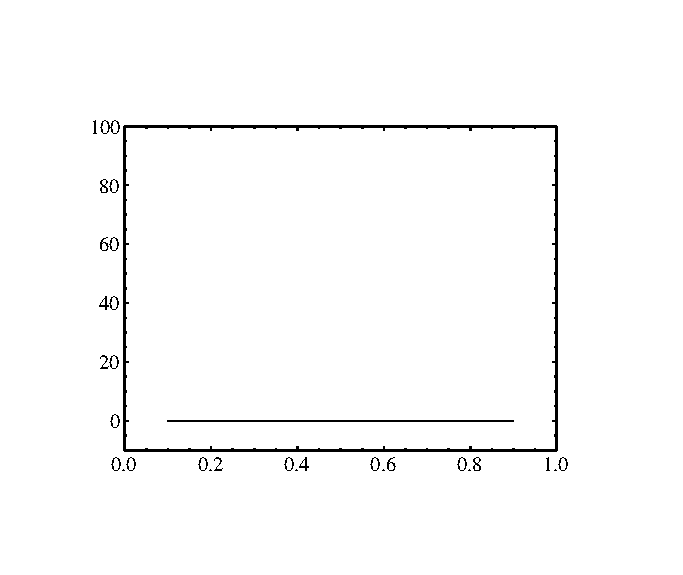
\includegraphics[width=0.5\textwidth]{FirstLevel.eps}
\caption{First level in SciDraw! \label{text:FirstLevel}}
\end{center}
\end{figure}
\newpage
Granted, this all seems like a lot of work just to draw a single horizontal line at {\tt y}=0, so let's add another level, ({\tt Lev$\llbracket``$162Dy$\_$2gs$"\rrbracket$[0,1,80];}) to get the output in Figure \ref{text:SecondLevel}:
\begin{figure}[h]
\begin{center}
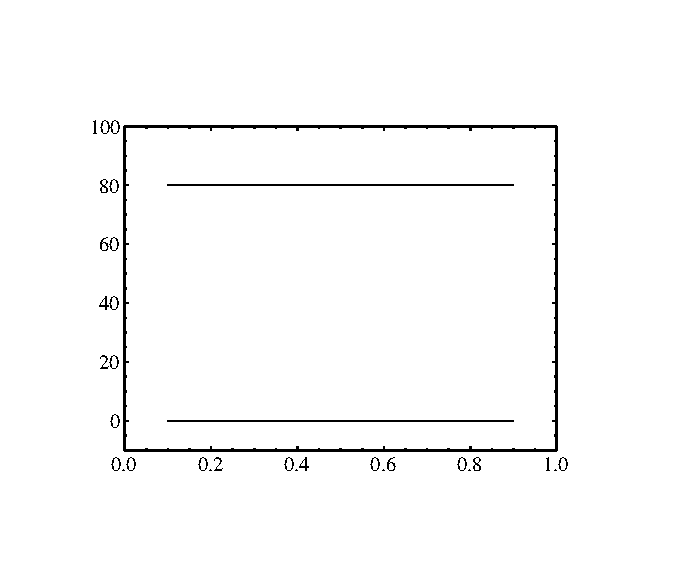
\includegraphics[width=0.45\textwidth]{SecondLevel.eps}
\end{center}
\caption{Second level being drawn in. \label{text:SecondLevel}}
\end{figure}

This is obviously not a pretty drawing, as it contains no label information or transitions, but a {\tt Lev} is the basis of all drawing done in SciDraw. The user can add any number of levels, given they have a discrete, unique name.
\subsection{Adding Transition Arrows to the Figure}
Drawing a transition arrow between two levels is simple; the {\tt Trans} command takes care of this, where the syntax is shown in equation \ref{eq:Trans}: 
\begin{equation} \label{eq:Trans}
{\tt Trans[``Parent\_Name",x_0,``Daughter\_Name",x_1,\textit{options}];}
\end{equation}
``{\tt Parent\_Name}" should be the name of the level you want to start from, similarly, ``{\tt Daughter\_Name}" is the name of the level you want the transition arrow to end at. {\tt x$_0$} is the position (relative to the start point of the level) at which the transition arrow should start on the parent level, with {\tt x$_1$} being the end position on the daughter level (again, relative to the level). {\tt x$_1$} can be a numerical value, or (in the vast majority of cases), one can use {\tt Automatic} to have SciDraw drop the transition arrow straight down. Again, \textit{options} clauses are purely optional, but will be discussed later. By adding:

\begin{figure}[h]
\begin{center}
   {\tt Trans}[``{\tt 162Dy\_2gs}",0.25,``{\tt 162Dy\_0gs}",{\tt Automatic}];\\
   {\tt Trans}[``{\tt 162Dy\_2gs}",0.50,``{\tt 162Dy\_0gs}",0.75];\\
\end{center}
To the body of the {\tt FigurePanel}, we produce:
\begin{center}
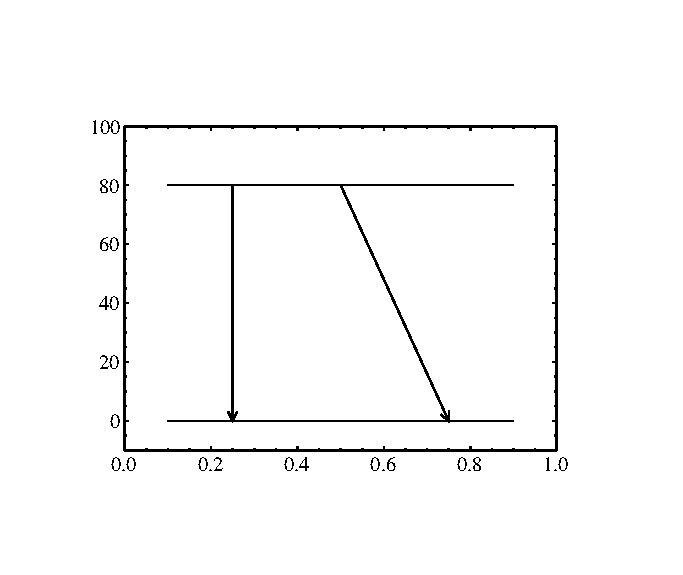
\includegraphics[width=0.5\textwidth]{Trans.eps}
\end{center}
\caption{Adding transition arrows in (straight down and from point-to-point). \label{text:Trans}}
\end{figure}

\subsection{Adding Text/Labels to the Figure}
Most labels and text are added as \textit{options} to either {\tt Lev} or {\tt Trans}; to add text, simply add:
\begin{equation}\label{eq:XLabel}
{\tt XLabel}\rightarrow``text"
\end{equation}

Where any \textit{options} would go. Here, the {\tt X} in {\tt XLabel} is one of five anchor points, {\tt Left}, {\tt Top}, {\tt Right}, {\tt Bottom}, or {\tt Center}. {\tt RightLabel} will make a label on the right side of the object to display whatever is in \textit{text}, which can be plain-text input, or a spin-parity assignment. Mathematica inputs do not adhere to the same standard of sub/superscripts that you may be used to; M. Caprio has aided the creation of spin-parity labels via {\tt LabelJP}. Typing {\tt LeftLabel$\rightarrow$LabelJP[2,+1]} as an \textit{option} for {\tt Lev} will place a 2$^+$ label on the left side of the named level. A standalone label (not as part of the \textit{options} of a command) for use is the {\tt BandLabel} command, which places a label under a named level at the midpoint of said level. The syntax for {\tt BandLabel} is:
\begin{equation} \label{eq:BandLabel}
{\tt BandLabel[}``{\tt Level\_Name}",``text",\textit{options}];
\end{equation}
Again, text can be plain-text input, or, another built-in SciDraw function (again due to the input limitations of Mathematica and superscripts), {\tt Isotope}. This is the easiest way to make atomic notation possible in SciDraw labels, by using:
\begin{equation}\label{eq:Isotope}
{\tt Isotope[}``{\tt A}", ``{\tt Nuclear\_Abbreviation}"]
\end{equation}
In {\tt Isotope}, take care not to forget the double quotations around each argument, where {\tt A} is the atomic mass number for a particular {\tt Nuclear\_Abbreviation}. Changing font sizes of labels is also done as part of the \textit{options} of a particular object via:
\begin{equation}\label{eq:FontSize}
{\tt FontSize\rightarrow VALUE}
\end{equation}
Where {\tt VALUE} is the numerical value (in printer point size) that you want the label's font to be displayed as. Refer to the included notebook walkthrough to see exact usages of labels, but a combination of all of the mentioned labels and options can be seen in figure \ref{text:Labels}:
\begin{figure}[h]
\begin{center}
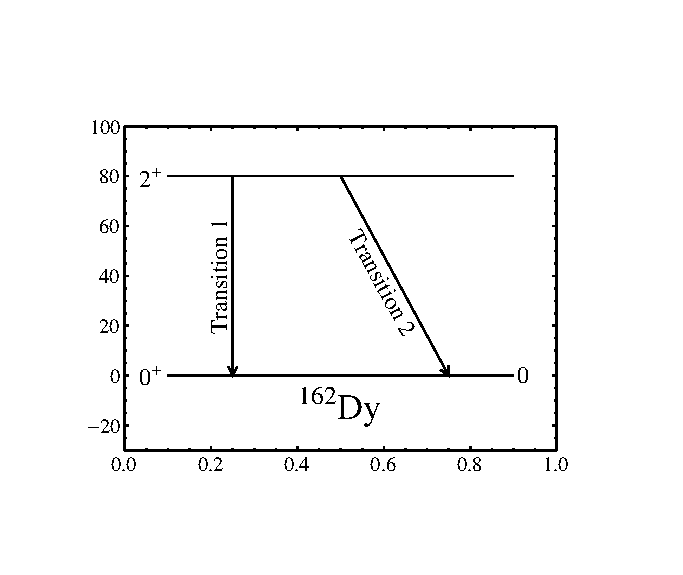
\includegraphics[width=0.5\textwidth]{Labels.eps}
\caption{Labels drawn on levels \& transitions, and {\tt Isotope} notation used in a {\tt BandLabel}. Note the increase in {\tt y}-axis range to account for the {\tt BandLabel}. \label{text:Labels}}
\end{center}
\end{figure}

%Automatic Energy Labels
\subsection{Commonly Used Options}
If the user grows tired of the default, simple line-style transition arrow, he/she can change this to be a thicker, block style transition arrow by using (\ref{eq:ArrowType}) as an \textit{option} for {\tt Trans}:
\begin{equation}\label{eq:ArrowType}
{\tt ArrowType\rightarrow Block}
\end{equation}
With this more robust arrow shape, the user can define several aspects of the {\tt Block ArrowType}. 

\begin{gather*}\label{eq:width}
{\tt Width\rightarrow VALUE}\\
{\tt HeadLength\rightarrow VALUE}
\end{gather*}


All allow the user to change the width of the arrow, as well as the length of the head. Measured in an absolute, arbitrary unit of measure, both {\tt Width} \& {\tt HeadLength} are defaulted to 5. 

SciDraw tends to follow the design philosophy of Henry Ford, in that the default color for any object is black. To help guide the eye, the user/reader can change the color of any object via \textit{options} on said object. Back on the splash screen of \ref{fig:splash}, M. Caprio has included the entire range of colors available to use in SciDraw. Colors of individual objects can be modified with:
\begin{equation}\label{eq:colors}
{\tt XColor\rightarrow COLOR}
\end{equation}
Similar to {\tt XLabel}, the {\tt X} in {\tt XColor} can reference multiple different objects, {\tt Font} (to change the color of font in labels for an object), {\tt Line} (to change the color of bounding lines for the {\tt Block ArrowType} or the color of a {\tt Lev}), {\tt Fill} (to change the interior color of the {\tt Block ArrowType}, among others (fully listed in M. Caprio's documentation). Following the {\tt Color} thread, the background color of text in a label (in either a level or transition label) can be changed (to add emphasis or aid readability) with:
\begin{equation}\label{eq:BackgroundColor}
{\tt TextBackground\rightarrow COLOR}
\end{equation}

If the default thickness (1 arbitrary unit) for a particular line or level is too thin, the user can change this thickness via:
\begin{equation}\label{eq:thickness}
{\tt LineThickness\rightarrow VALUE}
\end{equation}

Oftentimes, the text from multiple labels will overlap with other objects; the text anchoring system of SciDraw helps the user in that 
\begin{equation}\label{eq:TextNudge}
{\tt XTextNudge\rightarrow \{x,y\}}
\end{equation}
Where {\tt X} \textit{again} needs to reference the label object you want to nudge ({\tt Left, Right, Center}, etc.), and that {\tt \{x,y\}} specify the shift (in printer pts) horizontally to the right and vertically upward (take note that {\tt x \& y} can be negative). \textbf{A note from experience:} a great deal of time will be spent nudging labels to get precise placements and for small tweaks. Figure \ref{text:CommonOptions} is the output of many of the above options to change colors, font sizes, and arrow types. The user should refer to the included notebook to see the exact nature of each change provided.
\begin{figure}[h]
\begin{center}
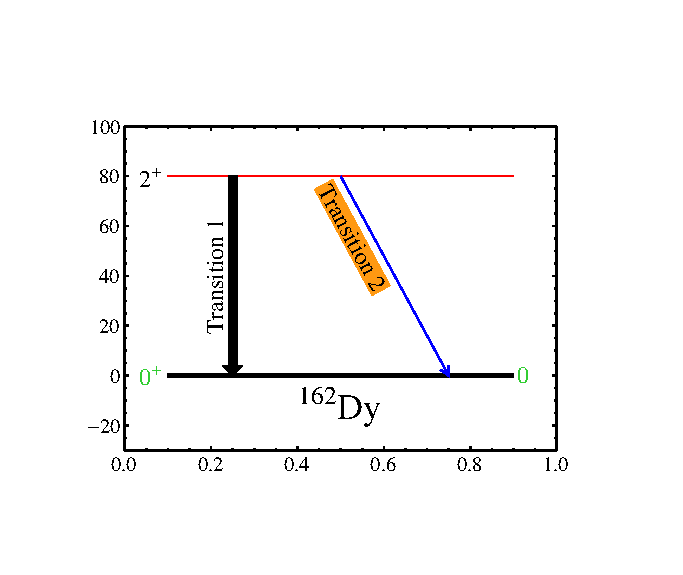
\includegraphics[width=0.45\textwidth]{CommonOptions.eps}
\caption{Various options being applied to levels, transitions, and labels \label{text:CommonOptions}}
\end{center}
\end{figure}

\subsection{Global Options and Frame Management}
If one of the particular \textit{options} need to be expressed in the majority of commands, the user can set global \textit{options} by declaring (at the top of the {\tt FigurePanel} body):
\begin{equation}\label{eq:TextNudge}
{\tt SetOptions[COMMAND},options];
\end{equation}
Any option that needs to be applied to all {\tt COMMAND}s of a particular type go in \textit{options}. For example, to make the font size 24 pt font for labels attached to a level, use {\tt SetOptions[Lev,FontSize$\rightarrow$24];}.
While the {\tt y}-axis is generally helpful to express the excitation energy of a level, oftentimes, the {\tt x}-axis holds no use for a final drawing. It is sometimes beneficial to leave it in to troubleshoot level or transition placements, but we can remove the {\tt x} axis from the frame with:
\begin{equation}\label{eq:XFrame}
{\tt XFrame\rightarrow False}
\end{equation}
In this case, {\tt X} does \textit{not} refer to a particular object, but instead just to remove the {\tt x}-axis (or {\tt y}-axis by using {\tt YFrame$\rightarrow$False}). An axis label can be placed on the {\tt y}-axis by invoking:
\begin{equation}\label{eq:YFrameLabel}
{\tt YFrameLabel\rightarrow}``text"
\end{equation}
These frame options are placed outside of the curly brackets of {\tt FigurePanel}, just after {\tt PlotRange}. Again, the supplementary notebook shows the exact usage of global options and the removal of the {\tt x}-axis, but the final output can be seen in figure \ref{fig:FinalOutput}:
\begin{figure}[h]
\begin{center}
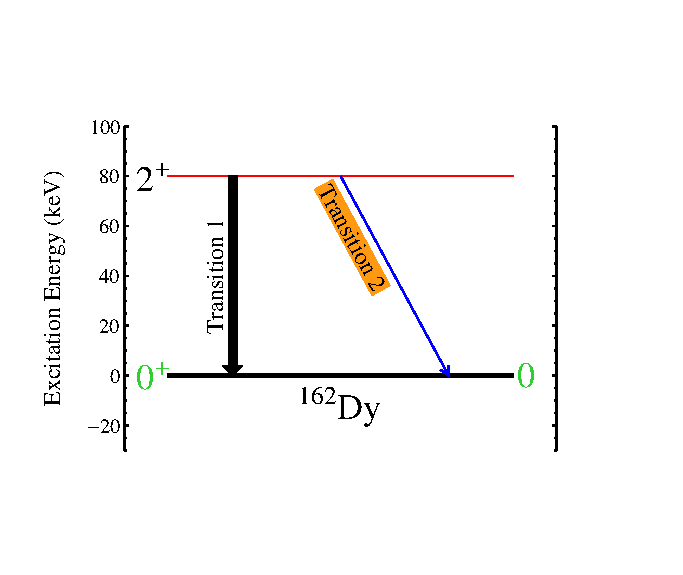
\includegraphics[width=0.45\textwidth]{FinalOutput.eps}
\caption{Global options applied to the font size on levels, a label placed on the {\tt y}-axis, and the removal of the {\tt x}-axis. \label{fig:FinalOutput}}
\end{center}
\end{figure}

Given the above examples, a working template, and the overview of the most basic of SciDraw functions, one can make a publication-quality level scheme with a very small amount of work. Exporting the level scheme to an ouput file is simple: just right-click the image output and select ``Save Graphic As..." to export to multiple image formats (\textit{.eps},\textit{.png}, etc.). Happy drawing!

\epigraph{``We don't make mistakes, we just have happy accidents."}{\textit{Bob Ross}\\The Joy of Painting (1983-1994)}

%\newpage
%\section{Quick-Reference of Syntax}


\end{document}